\documentclass[11pt]{article}
\usepackage{graphicx}
\usepackage{amsmath}
\usepackage{fullpage}
\usepackage{amssymb}
\usepackage{amsfonts}
\usepackage{latexsym}
\usepackage{algorithm}
\usepackage{algpseudocode}
\usepackage{natbib}
\usepackage{color}
\usepackage{multirow,bigstrut}
\usepackage{tabu}
\usepackage{array}
\usepackage{subcaption}
\usepackage{hyperref}


\newcommand {\R}    {{\rm I\!R}}
\newcommand {\bu}   { {\bf u} }   	% discrete flow field
\newcommand {\buref}   { {\bf u}_{\text{ref}} } % discrete reference flow field
\newcommand {\bugt}   { {\bf u}_{\text{gt}} } 	% discrete ground truth flow field

\newcommand {\vu}  { {\vec {\bf  u}} }   % continuous flow field
\newcommand {\vuref} {\vu_{\text{ref}}}  % continuous reference flow field
\newcommand {\vq}  { {\vec {\bf  q}} }
\newcommand {\ve}  { {\vec {\bf  e}} }
\newcommand {\vh}  { {\vec {\bf  h}} }
\newcommand {\vx}    {\vec {\bf x}}
\newcommand {\bx}    {{\bf{x}}}
\newcommand {\bflambda}    {{\boldsymbol{\lambda}}}
\newcommand {\blambda}	 { {\boldsymbol \lambda} }
\newcommand {\bmu}    	 { {\boldsymbol \mu} }
\newcommand {\zero}   	 { {\bf 0} }
\newcommand {\gb}      	 { {\bf g} }
\newcommand {\bnabla}	 { { \boldsymbol \nabla} }
\newcommand {\btheta}	 { { \boldsymbol \theta} }
\newcommand {\balpha}	 { { \boldsymbol \alpha} }
\newcommand {\bfxi}		 { { \boldsymbol \xi} }
\newcommand{\hx}[1]		{{\ensuremath{h^x_{\scriptscriptstyle #1}}}}
\newcommand{\hy}[1]		{{\ensuremath{h^y_{\scriptscriptstyle #1}}}}
\newcommand{\hz}[1]		{{\ensuremath{h^z_{\scriptscriptstyle #1}}}}
\newcommand{\E}			{\vec{E}}
\newcommand{\A}			{\vec{A}}
\renewcommand{\H}		{\vec{H}}
\newcommand{\J}			{\vec{J}}
\newcommand{\F}			{\vec{F}}
\newcommand{\M}			{\vec{M}}
\newcommand{\s}{\vec{s}}
\newcommand{\h}{\vec{h}}
\newcommand{\sig}{\sigma}
\renewcommand{\div}{\nabla\cdot\,}
\newcommand{\grad}{\ensuremath {{\bf{ \nabla}}}}
\newcommand{\curl}{\ensuremath{{\nabla}\times\,}}
\newcommand{\alert}[1] {\textcolor{red}{#1}}
\newdimen\iwidth\iwidth=30mm
	\newcommand{\rottext}[1]{\rotatebox{90}{\hbox to 30mm{\hss #1\hss}}}
\newcommand{\rme}{\rm{e}}
\newcommand{\HRule}{\rule{\linewidth}{0.25mm}}

\newcommand{\JJ}  {\mathcal{J}}    % objective functional
\newcommand{\cD}  {\mathcal{D}}    % data misfit
\newcommand{\CR}  {\mathcal{R}}    % regularization functional
\newcommand{\CRflow}  {\mathcal{R}^{\text{flow}}}    %  flow
\newcommand{\CRsat}   {\mathcal{R}^{\text{s}}}     %  saturation
\newcommand{\CF}  {\mathcal{F}}    % continuous tomography operator
\newcommand{\sh}  {\texttt{s}}     % discretized initial slowness
\newcommand{\DIVh}   {{\textsf{DIV}}}  % discretized divergence
\newcommand{\CURLh}  {{\textsf{CURL}}} % discrete curl operator
\newcommand{\GRADh}  {{\textsf{GRAD}}} % discrete gradient operator
\newcommand{\W}{\text{\bf W}}
\newcommand{\C}{\text{\bf C}}
\newcommand{\shat}{\widehat{s_0}}
\newcommand{\shatk}{\widehat{s}}
\newcommand{\mhat}{\widehat{\bf m}}
\newcommand{\what}{\widehat{\bf w}}
\newcommand{\Sig}{\bf \Sigma_m }
\newcommand{\Sigh}{\bf \Sigma}

\newcommand{\GRAD}{\nabla}
\newcommand{\DIV}{\nabla \cdot}


\newcommand{\deriv}[2]{\frac{\partial #1}{\partial #2}}
\newcommand{\diag}[1]{\text{ diag}\left(#1\right)}
\newcommand{\nn}{^{n+1}}
\newcommand{\nnm}{^{n+1,m}}
\newcommand{\nnmm}{^{n+1,m+1}}
\newcommand{\n}{^{n}}

\usepackage{xspace,color,amsmath}

\newcommand{\SimPEG}{\textsc{SimPEG}\xspace}

\newcommand{\bfA}{\mathbf{A}}
\newcommand{\bfB}{\mathbf{B}}
\newcommand{\bfC}{\mathbf{C}}
\newcommand{\bfD}{\mathbf{D}}
\newcommand{\bfE}{\mathbf{E}}
\newcommand{\bfF}{\mathbf{F}}
\newcommand{\bfG}{\mathbf{G}}
\newcommand{\bfH}{\mathbf{H}}
\newcommand{\bfI}{\mathbf{I}}
\newcommand{\bfJ}{\mathbf{J}}
\newcommand{\bfK}{\mathbf{K}}
\newcommand{\bfL}{\mathbf{L}}
\newcommand{\bfM}{\mathbf{M}}
\newcommand{\bfN}{\mathbf{N}}
\newcommand{\bfO}{\mathbf{O}}
\newcommand{\bfP}{\mathbf{P}}
\newcommand{\bfQ}{\mathbf{Q}}
\newcommand{\bfR}{\mathbf{R}}
\newcommand{\bfS}{\mathbf{S}}
\newcommand{\bfT}{\mathbf{T}}
\newcommand{\bfU}{\mathbf{U}}
\newcommand{\bfV}{\mathbf{V}}
\newcommand{\bfW}{\mathbf{W}}
\newcommand{\bfX}{\mathbf{X}}
\newcommand{\bfY}{\mathbf{Y}}
\newcommand{\bfZ}{\mathbf{Z}}

\newcommand{\bfa}{\mathbf{a}}
\newcommand{\bfb}{\mathbf{b}}
\newcommand{\bfc}{\mathbf{c}}
\newcommand{\bfd}{\mathbf{d}}
\newcommand{\bfe}{\mathbf{e}}
\newcommand{\bff}{\mathbf{f}}
\newcommand{\bfg}{\mathbf{g}}
\newcommand{\bfh}{\mathbf{h}}
\newcommand{\bfi}{\mathbf{i}}
\newcommand{\bfj}{\mathbf{j}}
\newcommand{\bfk}{\mathbf{k}}
\newcommand{\bfl}{\mathbf{l}}
\newcommand{\bfm}{\mathbf{m}}
\newcommand{\bfn}{\mathbf{n}}
\newcommand{\bfo}{\mathbf{o}}
\newcommand{\bfp}{\mathbf{p}}
\newcommand{\bfq}{\mathbf{q}}
\newcommand{\bfr}{\mathbf{r}}
\newcommand{\bfs}{\mathbf{s}}
\newcommand{\bft}{\mathbf{t}}
\newcommand{\bfu}{\mathbf{u}}
\newcommand{\bfv}{\mathbf{v}}
\newcommand{\bfw}{\mathbf{w}}
\newcommand{\bfx}{\mathbf{x}}
\newcommand{\bfy}{\mathbf{y}}
\newcommand{\bfz}{\mathbf{z}}

\newcommand{\hf}{\frac 1 2}

\newcommand{\bfdo}{\mathbf{d}_{\rm obs}}
\newcommand{\bfdp}{\mathbf{d}_{\rm pred}}



\newcommand{\bftheta}{\boldsymbol{\theta}}
\newcommand{\bfpsi}{\boldsymbol{\psi}}
\newcommand{\bfPsi}{\boldsymbol{\Psi}}


\newcommand{\FF}{F}


\def\kronecker{\raisebox{1pt}{\ensuremath{\:\otimes\:}}}
\sloppy


\author{Rowan Cockett, Supervisor:  Eldad Haber}
\begin{document}

\begin{titlepage}

\begin{center}

\textsc{\Large Ph.D. Thesis Proposal:}\\[0.5cm]

% Title
\HRule\\[0.01cm]
{ \huge \bfseries \linespread{5} \vspace{0.5cm} A Framework for Geophysical Inversions}\\%[1.9cm]
\HRule \\[0.75cm]
{\LARGE Rowan Cockett}\\[0.2cm]%
{\large May 04, 2016}\\[1.75cm]

% Authors
\begin{minipage}[t]{0.4\textwidth}
\begin{flushleft} \large
\emph{Supervisor:}\\
Eldad \textsc{Haber}\\[1.2cm]

\emph{Committee Members:}\\
Doug \textsc{Oldenburg}\\
Roger \textsc{Beckie}\\
[1.2cm]
\end{flushleft}
\end{minipage}
%
\begin{minipage}[t]{0.4\textwidth}
\begin{flushright} \large
\emph{External Examiner:} \\
Craig \textsc{Hart} \\[1.2cm]

\emph{Examination Chair:} \\
Douw \textsc{Steyn}
\end{flushright}
\end{minipage}

\vspace{3.5cm}

% Bottom of the page
\textbf{\large Department of Earth, Ocean and Atmospheric Sciences \\ [0.5cm]
\Large The University of British Columbia} \\[2.5cm]
\end{center}

\end{titlepage}


\newpage
%--------------------------------------------------------------------------------------
\tableofcontents
\newpage
%--------------------------------------------------------------------------------------
%--------------------------------------------------------------------------------------

\section{Introduction}
\label{sec:intro}

\subsection{Motivation}

The goal of the applied geosciences is to make predictions and decisions about the subsurface. The accuracy of these predictions can have far reaching economic and environmental implications (e.g. contamination delineation, resource exploration, reservoir optimization). There are many disciplines and skills that are involved in providing predictions and increasingly these disciplines must collaborate and integrate their domain specific knowledge.
In a managed aquifer recharge project, for example, the goal is to infiltrate water into the subsurface for storage and subsequent recovery. Throughout the lifetime of the project monitoring and management of the infiltration site is necessary (e.g. \cite{Racz2011,Daily1992,Park1998}). Such projects require input from geology, hydrology and geophysics to map the hydrostratigraphy, to collect and interpret time-lapse geophysical measurements, and to integrate all results to make predictions and decisions about fluid movement at the site.
The integration of the geosciences is far from trivial as each discipline has differing descriptive terminology as well as software tools that are domain specific with limited interoperability. Each of these domains involves their own physics problems and versions of discretization, regularization, optimization, computer science, empirical relations, and geology. In the geosciences, progress in integrating disciplines is hindered by an unformalized ontology and a history of proprietary software tools that have limited accessibility and poor interoperability. Geoscience integration is currently the target of major funding initiatives (e.g. EarthCube - 11 year NSF project, 35M in 2015; CIMIC Footprints Project - NSERC Project, 24 Universities, 30 Industry, 13M). Many of the current efforts are focused on software infrastructure, formally describing geoscientific data (using ontologies), and formally describing methods of integrating disciplines. Integration of disciplines and formally promoting quantitative communication throughout geophysical simulations and parameter estimation is crucial to integration; this is the main focus of my PhD.

\subsection{Geophysical inversion framework}

Geoscience inversions are the mathematical process of creating subsurface models to fit measured data, generally guided by physics. The language, workflow, and resulting software implementations of geoscience inversions varies across disciplines. These inconsistencies are among the large barriers to sustained cross-disciplinary integrations.
To address this barrier to geoscience integration, I strive to formalize geoscience inversions. This process will take the form of deriving, from the existing body of literature, a consistent terminology, a conceptual framework, and a software organization, which supports reproducible inversion workflows.
By formalize, I do not mean mathematically, rather taking practices of ontology and framework development in biology and other more mature interdisciplinary fields and applying them to geophysical inversions. In a Nature genetics review by \cite{Bard2004} the authors conclude: \emph{``An ontology makes explicit knowledge that is usually diffusely embedded in notebooks, textbooks and journals or just held in academic memories, and therefore represents a formalization of the current state of a field.''}.
Adapting these methodologies to geophysical inversions inherently requires that a diverse suite of methods and applications be considered across geophysics, hydrogeology and geology. The geoscience problems that I am using to illuminate this work are: direct current resistivity \citep{Cockett2014a,Pidlisecky2013,Steklova2012}, frequency/time domain electromagnetics \citep{Kang2014,Heagy2015,Fohring2012,Kang2015}, vadose zone fluid flow (Cockett \& Haber, in prep), and parameterized geologic modeling \citep{Cockett2016,Cockett2013b,Cockett2012}.
The way in which I am working to formalize geoscience inversions is through the development of a rigorously tested framework that supports and enables these works. Each of these problems has its own unique constraints: each has its own physics and physical properties, empirical relations may be considered, requirements on the spatial and temporal discretizations, large matrix systems to solve with variable structure and possibly with many sources, and unique parameterizations that are context specific for a geoscience decision.

The initial version of the framework was published in Computers and Geoscience \citep{Cockett2015}, a brief illustration of the major components and layout of the framework is seen in Figure~\ref{fig:simpeg}, for a more in depth discussion, please refer to the paper, the online documentation (\url{http://docs.simpeg.xyz}) or the primary open-source numerical implementation (\url{https://github.com/simpeg/simpeg}).
The framework has since been extended, refined and used for research problems in: induced polarization \citep{Kang2016}, electromagnetics (Heagy, Cockett, et al; in prep), magnetotellurics (Rosenkjaer et al. in prep, \cite{Rosenkjaer2015AGU}), gravity, magnetics, and seismic, as well as a number of other conference proceedings \citep{Cockett2015a,Rosenkjaer2015}. The framework and software has also seen use in industry applications, as well as university courses and training \citep{Heagy2015b,HeagySciPy2015}, in reproducible textbooks (http://em.geosci.xyz, http://gpg.geosci.xyz), has seen multiple awards (UBC Library Award, NSERC Doctoral Prize for Interdisciplinary Research) and will be the subject of an upcoming conference (BIRS - Geophysical Simulation and Inversion, August 2016).

\begin{figure}[ht!]
\centering
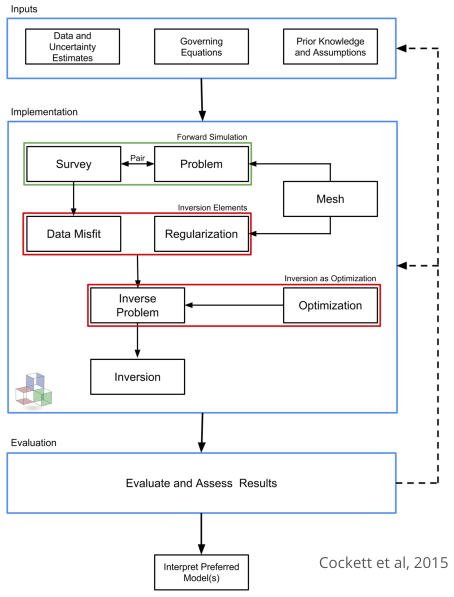
\includegraphics[width=10cm]{simpegFramework.png}
\caption{Illustration of the \SimPEG framework showing the major components and their interconnectivity. Adapted from \cite{Cockett2015} (\href{http://creativecommons.org/licenses/by/4.0/}{CC-BY-4.0}).}
\label{fig:simpeg}
\end{figure}

I plan to address and further develop this framework through two avenues:
\begin{enumerate}
\item vadose zone inverse problems using Richards equation with careful attention to the computational scalability of the parameter estimation problem;
\item integration of simple process based geologic parameterizations with the geophysics framework to support geologic interpretation of geophysical data.
\end{enumerate}
Additionally, in collaboration with Heagy, Kang, Rosenkjaer and Oldenburg I will extend and refine the framework to support electromagnetic inversions in a variety of formulations and applications of steel casing and geothermal exploration. The work on the electromagnetics framework is to be submitted by June 2016 to Geophysics. These research areas may seem disparate, but collectively they are united by a common theme of addressing the complexities of bringing together the disciplines of geophysics, hydrology, geology, and inverse theory in a computationally tractable manner that is accessible and reproducible by other researchers. In this proposal I will provide a brief background on geophysical inverse problems and vadose zone flow, highlighting the need for computational feasibility and a framework to support simulation and inversion across multiple disciplines.

Throughout this work, my colleagues and I have tried to summarize and/or reproduce a large quantity of the geophysical inversion literature. This has been difficult due to the diverse terminology describing extremely similar methodologies and a lack of numerical instructions (often intentionally withheld). This proprietary paradigm does not enable the diverse collaborations necessary for geoscience integration. I have looked to and learned from other fields (e.g. biology, astrophysics, machine learning  \cite{Astropy,scikit-learn}) on how to organize a community around open, accessible, actionable ideas. Adapting these learnings to geoscience, I strive to complete all of my research such that it is immediately reproducible and openly available \citep{Cockett2015c,Wilson2014, RTFD, Travis, Coveralls}. Much of my work requires software, which is `implementation' and `engineering' by its nature. However, the software (although extremely useful) is not the aim of my research: software is the means by which I test, extend, and generalize my ideas in a rigorous, scientific way. The aim of my research is to identify, explore, and formalize a framework for simulation and parameter estimation in geophysics.

\subsection{Application to vadose zone fluid flow}

The development of a geophysical framework requires considering a number of disciplines and geophysical problems to ensure generality as well as extensibility. I am working with collaborators in many of these geophysical methods (electromagnetics, direct current resistivity, magnetotellurics, magnetics, gravity) and am ensuring that the framework that I am developing supports these applications. However, the goal is also to have the framework work outside of geophysics and most notably in hydrogeology, as such, I have chosen vadose zone fluid flow as a model problem. Additionally, there are a few numerical techniques which I have identified that would be a significant contribution in the context of hydrogeophysical inversions. Fluid flow in the vadose zone is governed by Richards equation and parameterized by hydraulic conductivity, which is a nonlinear function of pressure head. Investigations in the vadose zone typically require identification of distributed hydraulic properties. This is increasingly being done through a data-driven approach, using changes in saturation or pressure head to infer hydraulic parameters. Hydrogeophysics allows many more proxy measurements, such as direct current resistivity data, to be taken to help characterize these sites spatially, as well as through time. As such, the number of distributed hydraulic parameters to be estimated in a Richards equation inversion will continue to grow. There has been much research into the scalability of the inverse problem in geophysical applications (e.g. electromagnetics) that allow the calculation of an optimization step in the inversion \emph{without} explicitly calculating or storing the sensitivity matrix (cf. \cite{hao}). This is extremely important in large problems as the computer memory available to store this large, dense matrix can often be a limitation. Previous work use either numerical differentiation, automatic differentiation, or finite difference in order to compute the sensitivity matrix (e.g. PEST) \citep{Finsterle2011c, Bitterlich2002}. This is computationally slower and can generate inaccuracies in the sensitivity computation and tarry convergence of the optimization algorithm. With regard to implicit sensitivity calculations, there is an opportunity to apply some of the learnings from the geophysical inversion literature to this hydrogeologic problem. Note that the sensitivity calculation is necessary in \emph{any} gradient based technique.

The application of the implicit sensitivity calculation to Richards equation, however, is not straightforward. Hydraulic conductivity is the function we are inverting for - it is an empirical function that depends on pressure head - pressure head is the field that is calculated using Richards equation. This nonlinear coupling requires iterative optimization methods in the forward simulation between each time step (e.g. Picard or Newton). This makes the implicit calculation of the effect of the sensitivity on a vector rather involved and intricate. Furthermore, the nonlinear relationship of hydraulic conductivity is empirically determined and depending on the relation used could involve the estimation of up to nine spatially-distributed parameters from a finite dataset. The implicit use of the sensitivity matrix should have the ability to calculate the sensitivity to any of these model parameters, however, any inversion algorithm would be ill-advised to try to estimate all distributed parameters at once. One goal of the proposed work is to tackle the sensitivity calculation \emph{implicitly}. This would further allow for exploration into different inversion methodologies and parameterizations of the empirical relationships. By not storing the sensitivity, and instead computing its effect on a vector, the size of the problem that we can invert will become much larger. This will allow large 3D hydraulic parameter inversions using Richards equation to be run on modest computational resources. Below is a brief mathematical sketch of the implicit sensitivity calculation. The full derivation as well as the numerical implementation are to be submitted in June 2016 to Inverse Problems.

\section{Geophysical inverse problems}

\subsection{Background and motivation}

Geophysical surveys can be used to obtain information about the subsurface as the responses that are measured depend on the physical properties and contrasts in the earth. Inversions provide a mathematical framework for constructing subsurface models consistent with the data collected by these surveys. The data collected are finite in number while the physical property distribution of the earth is continuous. Thus, inverting for a physical property model from geophysical data is an ill-posed problem, meaning that no unique solution explains the data. Furthermore, the data may be contaminated with noise. Therefore, the goal of a deterministic inversion is not only to find a model consistent with the data, but must be to find the `best' model that is consistent with the data. The definition of `best' requires the incorporation of assumptions and \emph{a priori} information, often in the form of an understanding of the particular geologic setting or structures \citep{Constable1987, DougTutorial, lelievre2009integrating}. Solving the inverse problem involves many moving pieces that must work together, including physical simulations, optimization, linear algebra, and incorporation of geology. Deterministic geophysical inversions have been extensively studied, and many components and methodologies have become standard practice. With increases in computational power and instrumentation quality, there is a greater drive to extract more information from the geophysical data. Additionally, geophysical surveys are being applied in progressively more challenging environments. As a result, the geosciences are moving towards the integration of geological, geophysical, and hydrological information to better characterize the subsurface (e.g. \citep{ho,Doetsch2010,Gao2012}). This is a scientifically and practically challenging task \citep{Li2000a, lelievre2009integrating}. These challenges, compounded with inconsistencies between different data sets, often makes the integration and implementation complicated and/or non-reproducible. The development of new methodologies to address these challenges will build upon, as well as augment, standard practices; this presupposes that researchers have access to consistent, well-tested tools that can be extended, adapted and combined.

There are many proprietary codes available that focus on efficient algorithms and are optimized for a specific geophysical application (e.g. \citep{Kelbert2014a, Key2007, liol96, Li1998a}). These packages are effective for their intended application, for example, a domain specific large-scale geophysical inversion or a tailored industry workflow. However, many of these packages are `black-box' algorithms, that is, they cannot easily be interrogated or extended. As researchers, we require the ability to interrogate and extend ideas; this must be afforded by the tools that we use. Accessibility and extensibility with regard to the geoscience application are the primary motivators for my work. Other disciplines have approached the development of these tools through open source initiatives using interpreted languages, for example, Astropy in astronomy \citep{Astropy} and SciPy in numerical computing \citep{scipy}. Interpreted languages facilitate interactive development using scripting, visualization, testing, and interoperability with code in compiled languages and existing libraries. Furthermore, many open source initiatives have led to communities with hundreds of researchers contributing and collaborating using social coding platforms, such as GitHub (https://github.com). There are also initiatives in the geophysical forward and inverse modeling community targeting specific geophysical applications (cf. \citep{Hansen2013, PySIT2013, Uieda2014, Kelbert2014a, Modflow}). I am interested in creating a community around geophysical simulations and gradient based inversions that is contributing to a consistent body of knowledge. To create a foundation on which to build a community, we require a comprehensive framework that is applicable across domains and upon which researchers can readily develop their own tools and methodologies. To support these goals, this framework must be modular and its implementation must be easily extensible by domain specific researchers.

\subsection{Take home points}
Sustained, reproducible integration requires that methodologies be accessible, consistent, numerically documented, interoperable and extensible. To do this, research is required to:
\begin{itemize}
    \item Identify the pieces and interfaces
    \item Abstract commonalities to a consistent, supporting subset
    \item Capture heuristics in a reproducible manner
    \item Numerically test, capture and document
\end{itemize}
The output of this will be a conceptual framework that is numerically tested and demonstrates the capability to support existing and future research directions, and will ideally catalyze and accelerate interdisciplinary collaborations.

\section{Vadose Zone Flow}

\subsection{Motivation}

Studying the processes that occur in the vadose zone, the region between the earth's surface and the fully saturated zone, is of critical importance for the understanding of our groundwater resources. The majority of groundwater recharge is derived through water that percolates through the vadose zone. As such, much attention has been given to monitoring and describing processes that reside in this region of the earth. Flow in the vadose zone is regulated by hydraulic conductivity, which is a non-linear function of saturation. This non-linear function is defined empirically using, for example, the Brooks-Corey model \citep{Brooks1964} or the van Genuchten-Mualem model \citep{Mualem1976,VanGenuchten1980}. Typically, the hydraulic conductivity is heterogeneous and can have large dynamical range. The spatial estimation of the hydraulic conductivity function is an important step in any site characterization; however, this estimation is difficult and simplifications are consistently used to avert these conceptual and computational difficulties. These simplifications typically parameterize the conductivity and assume that it is a simple function in space (e.g. \cite{Liang2014}). Such assumptions are often sufficient to fit observed (or conceptual) measurements because of the lack of constraining data, especially in two- and three-dimensions as well as in time. As more data becomes available through spatially extensive surveys, and time-lapse proxy measurements (e.g. direct current resistivity surveys, distributed temperature sensing) the possibility to extract more information about subsurface hydrogeologic parameters becomes a possibility. Fluid flow in the vadose zone is governed by Richards equation and parameterized by hydraulic conductivity, which is a non-linear function of pressure head. Recent advancements have been made to simulate Richards equation in a computationally scalable manner \citep{RichardsFOAM}. However, the inverse problem is non-trivial, especially in three-dimensions, and must be considered using modern numerical techniques that allow for spatial estimation of hydraulic parameters.

\subsection{Background}

Flow in the vadose zone has many complications as the parameters that control the flow are dependent on the saturation of the media, leading to a non-linear problem. The groundwater flow equation has a diffusion term, as well as an advection term that is related to gravity and only acts in the $z$-direction. There are two different forms of Richards equation that differ on how they deal with the non-linearity in the time-stepping term. Here we use the most fundamental form, referred to as the `mixed'-form of Richards equation \citep{Celia1990}:
\begin{equation}
\label{eq:RichardsMixed}
    \frac{\partial \theta(\psi)}{\partial t} - \DIV k(\psi) \GRAD \psi - \frac{\partial k(\psi)}{\partial z} = 0
    \quad \psi \in \Omega
\end{equation}
\noindent
where $\theta$ is water content, and $\psi$ is pressure head. This formulation of Richards equation is called the `mixed'-form because the equation is parameterized in $\psi$ but the time-stepping is in terms of $\theta$. The hydraulic conductivity, $k(\psi)$, is heterogeneous and potentially anisotropic function that is assumed to be given when solving the forward problem. In the following equations we assume that $k$ is isotropic, but the extension to anisotropy is straightforward and is completed numerically. The equation is solved in a domain $\Omega$ equipped with boundary conditions on $\partial \Omega$ and initial conditions that are problem dependent.

An important aspect of unsaturated flow is noticing that both water content, $\theta$, and hydraulic conductivity, $k$ are functions of pressure-head, $\psi$. There are many empirical relations used to relate these parameters, including the Brooks-Corey model \citep{Brooks1964} and the van Genuchten-Mualem model \citep{Mualem1976,VanGenuchten1980}. The van Genuchten model is written as:
\begin{subequations}
\label{eq:vanGenuchten}
\begin{equation}
\label{eq:theta_h}
    \theta(\psi) =
    \left\{\begin{aligned}
        \theta_r& + \frac{\theta_s- \theta_r}{(1+|\alpha \psi|^n)^m}  & \psi < 0 \\
        \theta_s& & \psi \ge 0
    \end{aligned}\right.
\end{equation}
\begin{equation}
\label{eq:K_h}
    k(\psi) =
    \left\{\begin{aligned}
        K_s & \theta_e(\psi)^l(1-(1- \theta_e(\psi)^{-m})^m)^2 & \psi < 0 \\
        K_s& & \psi \ge 0
    \end{aligned}\right.
\end{equation}
\end{subequations}
where
\begin{equation}
\label{eq:vanGenuchtenParams}
    \theta_e(\psi) = \frac{\theta(\psi) - \theta_r}{\theta_s - \theta_r},
    \qquad
    m=1- \frac{1}{n},
    \qquad
    n > 1
\end{equation}
Here $\theta_r$ and $\theta_s$ are the residual and saturated moisture contents; $K_s$ is the saturated hydraulic conductivity; $\alpha$ and $n$ are fitting parameters; and $\theta_e(\psi) \in [0,1]$ is the effective saturation. The pore connectivity parameter, $l$, is often taken to be $\frac{1}{2}$ as determined by \citep{Mualem1976}. Small changes in pressure head can change the hydraulic conductivity several orders of magnitude; as such, $k(\psi)$ is a highly nonlinear function and this makes Richards equation a highly nonlinear parabolic partial differential equation.

\subsection{Implicit sensitivity through matrix-vector products}

An efficient solution of the optimization problem requires
the derivative of the pressure head at all times, $\bfPsi$, with respect to the model parameters $\bfm$,
the so called, sensitivity matrix, $\bfJ$.
An approximation of the sensitivity matrix
can be obtained by using a finite difference method on the forward
problem \citep{Simunek1996,Finsterle2011,Finsterle2011c}. One forward problem,
or two when using central differences, must be completed for each column in
the Jacobian at every iteration of the optimization algorithm. This
differentiation has the advantage that it can be applied to any forward
problem, however, it is highly inefficient and introduces errors into the
inversion that may slow the convergence of the scheme. Automatic differentiation
(AD) can also be used \citep{nw} however, AD yields a dense Jacobian and does
not take the structure of the problem into consideration.
\cite{Bitterlich2002} presents three algorithms (finite difference, adjoint, and direct) to
directly compute the elements of the dense sensitivity matrix for Richards equation.
As we show next, it is possible to
explicitly write the derivatives of the Jacobian and evaluate their products with vectors.
This is a much more efficient
algorithm compared with finite differencing or AD, especially for large scale simulations, since it does not require storing
a large and dense matrix and can be used in order to efficiently compute matrix-vector
and adjoint matrix vector products.
These products can be used for the solution of the Gauss-Newton system when using the conjugate gradient method.
The idea has been used extensively for other inverse problems \citep{hao}. The challenge in
implementing it for Richards equation lies in differentiating the nonlinear forward problem with respect
to the hydraulic parameters. However, as we show next, this can be completed even for
highly nonlinear parameterizations, by using implicit differentiation and the chain rule.

\bigskip

The derivative of Richards equation in time involves writing the whole time-stepping
process as a block-matrix and taking the derivative. The discrete
Richards equation can be written as a function of the model, and for one
time-step is written:
\begin{equation}
\label{eq:Richards}
\FF(\bfpsi\nn,\bfpsi\n,\bfm) =
\frac{\bftheta\nn(\bfpsi\nn) - \bftheta^n(\bfpsi\n)}{\Delta t}
+
\bfD \diag{\bfk_{Av}(\bfpsi\nn,\bfm)}\bfD^{\top} \bfpsi\nn
+
\bfD_{z} \bfk_{Av}(\bfpsi\nn,\bfm)
= 0
\end{equation}
In this case $\bfm$ contains all the parameters of interest and is a vector. Here
we note that $\bfpsi\nn$ and $\bfpsi\n$ are also functions of $\bfm$. The derivatives
of $\FF$ to the change in the parameters $\bfm$ can be written in general as
\begin{equation}
\label{eq:sensitivity}
    \GRAD_\bfm  F(\bfpsi^n,\bfpsi\nn,\bfm)
    =
    \deriv{F}{\bfk_{Av}}\deriv{\bfk_{Av}}{\bfm}
    + \deriv{F}{\bfpsi^n}\deriv{\bfpsi^n}{\bfm}
    + \deriv{F}{\bfpsi\nn}\deriv{\bfpsi\nn}{\bfm}
    =0
\end{equation}
or in more detail
\begin{align}
\frac{1}{\Delta t}
\left(
    \deriv{\bftheta\nn}{\bfpsi\nn}\deriv{\bfpsi\nn}{\bfm}
    -
    \deriv{\bftheta\n}{\bfpsi\n}\deriv{\bfpsi\n}{\bfm}
\right)
+
\bfD \diag{\bfD^{\top} \bfpsi\nn}
    \left(
        \deriv{\bfk_{Av}}{\bfm} + \deriv{\bfk_{Av}}{\bfpsi\nn}\deriv{\bfpsi\nn}{\bfm}
    \right)
\nonumber\\
+\
\bfD \diag{\bfk_{Av}(\bfpsi\nn)} \bfD^{\top} \deriv{\bfpsi\nn}{\bfm}
+
\bfD_{z}^{\top}
\left(
    \deriv{\bfk_{Av}}{\bfm} + \deriv{\bfk_{Av}}{\bfpsi\nn}\deriv{\bfpsi\nn}{\bfm}
\right)
=0
\end{align}
The sensitivity matrix is the derivatives of $\bfPsi$ to $\bfm$ and the above equation
can be viewed as a system of linear equations for its estimation.
To solve for $\deriv{\bfPsi}{\bfm}$ we rearrange the
above equation into a block-matrix.
\begin{align}
\label{eq:rearrangedDeriv}
\overbrace{
\left[
    -\frac{1}{\Delta t} \deriv{\bftheta\n}{\bfpsi\n}
\right]
}^{\bfA_{-1}(\bfpsi\n)}
\deriv{\bfpsi\n}{\bfm}
+
&
\overbrace{
    \left[
        \frac{1}{\Delta t} \deriv{\bftheta\nn}{\bfpsi\nn}
        +\bfD \diag{\bfD^{\top} \bfpsi\nn}\deriv{\bfk_{Av}}{\bfpsi\nn}
        +\bfD \diag{\bfk_{Av}(\bfpsi\nn,\bfm)} \bfD^{\top}
        + \bfD_{z}\deriv{\bfk_{Av}}{\bfpsi\nn}
    \right]
}^{\bfA_0(\bfpsi\nn)}
\deriv{\bfpsi\nn}{\bfm}
\nonumber\\
=
&
\underbrace{
\bfD \diag{\bfD^{\top} \bfpsi\nn}\deriv{\bfk_{Av}}{\bfm}
+\bfD^{\top}_{z}\deriv{\bfk_{Av}}{\bfm}
}_{\bfB(\psi\nn)}
\end{align}
Here, we use the subscript notation of $\bfA_0(\bfpsi\nn)$ and
$\bfA_{-1}(\bfpsi\n)$ to represent two diagonals of the large sparse block-matrix
$\bfA({\bfPsi},\bfm)$.
% Note that all the terms in these matrices are already evaluated when computing
% the Jacobian of Richard's equations in Section~\ref{secForward} and that they
% contain only basic sparse linear algebra manipulations without the inversion of any matrix.
If $\bfpsi_0$ does not depend on the model, meaning
the initial conditions are independent, then the block system can be
formulated as:
\begin{equation}
\label{eq:jacobian_Time}
\overbrace{
    \left[
    \begin{array}{cccccc}
        \bfA_0(\bfpsi_1)&&&\\
        \bfA_{-1}(\bfpsi_1)&\bfA_0(\bfpsi_2)&&\\
        &\bfA_{-1}(\bfpsi_2)&\bfA_0(\bfpsi_3)&\\
        &&\ddots&\ddots&&\\
        &&&\bfA_{-1}(\bfpsi_{n_{t}-1})&\bfA_0(\bfpsi_{n_{t}})\\
    \end{array}
    \right]
}^{\bfA(\bfPsi,\bfm)}
\overbrace{
    \left[
    \begin{array}{c}
        \deriv{\bfpsi_1}{\bfm}\\
        \deriv{\bfpsi_2}{\bfm}\\
        \vdots\\
        \deriv{\bfpsi_{n_{t}-1}}{\bfm}\\
        \deriv{\bfpsi_{n_{t}}}{\bfm}\\
    \end{array}
    \right]
}^{\deriv{\bfPsi}{\bfm}}
    =
\overbrace{
    \left[
    \begin{array}{c}
        \mathbf{B_1}(\bfpsi_1)\\
        \mathbf{B_2}(\bfpsi_2)\\
        \vdots\\
        \mathbf{B_{n-1}}(\bfpsi_{n_{t}-1})\\
        \mathbf{B_n}(\bfpsi_{n_{t}})\\
    \end{array}
    \right]
}^{\bfB(\bfPsi,\bfm)}
\end{equation}
This is a block matrix equation, and both the storage and
solving will be expensive if it is explicitly computed. Indeed, its direct
computation is equivalent to the adjoint method previously discussed.

However, since only matrix vector products are needed for the inexact Gauss-Newton optimization
method the  matrix $\bfJ$ is never
needed explicitly  and only the products of the form $\bfJ \bfv$ and
$\bfJ^\top \bfz$ are needed, for arbitrary vectors $\bfv$ and $\bfz$.
Projecting the full sensitivity
matrix onto the data-space using $\bfQ$, results in the following
equations for the Jacobian:
\begin{subequations}
    \begin{equation}
    \label{eq:jacobian_Multiplication}
        \bfJ = \bfQ \bfA(\bfPsi,\bfm)^{-1} \bfB(\bfPsi,\bfm)
    \end{equation}
    \begin{equation}
    \label{eq:jacobianT_Multiplication}
        \bfJ^\top =   \bfB(\bfPsi,\bfm)^\top \bfA(\bfPsi,\bfm)^{-\top} \bfQ^\top
    \end{equation}
\end{subequations}
\noindent
In these equations we are careful to not write $\deriv{\bf\Psi}{\bfm}$, as it is
a large dense matrix which we do not want to explicitly compute or store.
Additionally, the matrices $\bf A(\bfPsi,\bfm)$ and $\bf B(\bfPsi,\bfm)$ do not even
need to be explicitly formed because the matrix $\bf A(\bfPsi,\bfm)$ is a
triangular block-system, and can be solved using forward or backward
substitution, with only one block-row being solved at a time.
To compute the matrix vector product $\bfJ \bfv$ we use a simple
algorithm:
\begin{enumerate}
    \item Given the vector $\bfv$ calculate $\bfy = \mathbf{Bv}$
    \item Solve the linear system $\mathbf{Aw} = \bfy$ for the vector $\bfw$
    \item Set $\bfJ \bfv = \bfQ \bfw$
\end{enumerate}
Here we note that steps (1) and (2) are actually done using a for-loop with
only one row being computed and stored at a time. As such, only the full
solution, $\bf \Psi$, is stored and all other block-entries may be
computed as needed. Similarly, to compute the adjoint
$\bfJ^\top \bfz$ involves the intermediate solve for $\bfy$
in $\bfA^\top \bfy = \bfQ^\top \bfz$ and then
computation of $\bfB^\top \bfy$. Again, the block-matrix solve is
done via backward substitution with all block matrix entries being computed as
needed.
Note that the backward substitution algorithm can be viewed as time stepping, starting
from the final time back to the initial time. This is equivalent to the adjoint method that
is discussed in \cite{DeanChen2011} and reference within. The main difference between
our approach and the classical adjoint based method is that our approach yields the {\em exact}
gradient of the discrete system; no such guaranty is given for adjoint based methods.

\subsection{Take home points}

\begin{itemize}
    \item Need computational scalability when moving to large 3D distributed parameter estimation.
    \item Implicit sensitivities are a part of the solution to the scalability.
    \item Parameterizations of the empirically determined hydraulic conductivity function $k(\psi)$:
    \begin{itemize}
        \item needs reduction of the parameter space to be estimated, and
        \item should be geologically motivated.
    \end{itemize}
\end{itemize}


\begin{figure}[ht!]
\centering
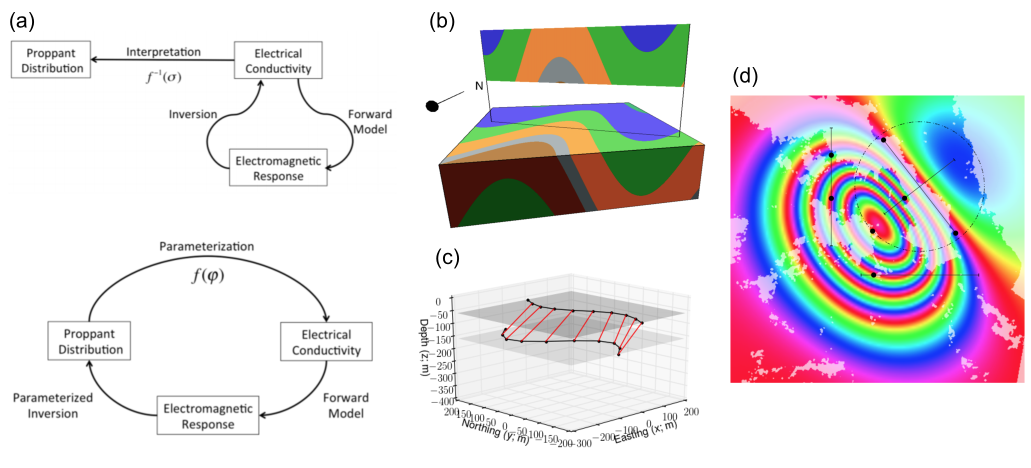
\includegraphics[width=16cm]{parameterizations.png}
\caption{Four examples of geologic and a-priori parameterizations: (a) parameterizing a proppant distribution using effective medium theory \citep{HeagySEG2014}, (b) process based geologic parameterizations \citep{Cockett2016}, (c) interface detection of a seawater intrusion using frequency domain electromagnetics \citep{KangSEG2015}, and (d) earthquake parameter estimation using InSAR data and a linear elastic dislocation \citep{Cockett2014b}.}
\label{fig:parameterizations}
\end{figure}

\section{Interfacing to geologic and a-priori information}

Incorporating and quantitatively communicating a-priori and geologic information is a perennial problem in geophysics.
There are many existing solutions for inclusion of this information into geophysical inversions, often these methods are completed through parameterizations (e.g. \cite{Oldenburga,Li1998a,liol96,Pidlisecky2007,Pidlisecky2011,McMillan2015}). However, each  decision, prediction, and geologic setting is unique: each will often require a new parameterization. I have been involved in a body of work that is researching instances of these parameterizations including: parameterized inversion for proppant distribution in fractures \citep{HeagySEG2014}, a parameterized model for linear elastic earthquake modelling \citep{Cockett2014b}, inverting for seawater intrusion interfaces \citep{Kang2015}, and a simple geologic parameterization algorithm \citep{Cockett2016,Cockett2013b,Cockett2012} (Figure~\ref{fig:parameterizations}). The goal of these works is to understand and abstract these parameterizations into a subset of methods that can generally support the abstract classes of parameterizations. This is an important aspect of an inversion framework: it must have the flexibility to support and interface to arbitrary parameterizations.


A general architecture requires that derivatives be calculated with respect to: (a) multiple physical properties (e.g. electrical conductivity, hydraulic conductivity, magnetic permeability), (b) the geophysical sources (e.g. waveform, transmitter location), and (c) the receivers (e.g. location, orientation).
In order to support the custom parameterizations that are necessary for a unique decision or prediction, this architecture must provide building blocks that are independently extensible. Using examples from multiple fields, including electromagnetics, fluid flow, and parameterized geologic modeling, I plan to investigate the abstractions necessary to simultaneously support a breadth of custom parameterizations.



\section{Research questions and thesis outline}

Based on the current state of the geoscience inversion community and the observations outlined above, I will arrange my thesis to address three key research topics: (1) developing an extensible framework for geophysical inversions, (2) computationally scalable vadose zone parameter estimation, (3) interfacing to geologic and a-priori information through parametrizations. The overarching goal is to promote integration between the geoscience disciplines; this has guided much of my work. Interdisciplinary integration requires reproducibility, accessibility, and collaboration, as such these are crucial to my work and demonstrated throughout. The research topics that I propose are:


\subsection{Simulation and Parameter Estimation Framework}

\noindent
{\bf Problem}

\noindent
Geophysical methods for simulation and parameter estimation in geophysics are often treated independently, especially in software, leading to poor interoperability between researchers. This hinders integrations and explorations into combining methods. The terminology and layout of ideas is disorganized internal to and between geophysical and hydrogeologic disciplines, which leads to slow transfer of new ideas. There are no openly available frameworks for geophysical inversions that are independently extensible (i.e. glass-box extensibility).

\noindent
{\bf Question}

\noindent
What is the structure, interconnectivity and architecture of a framework for geophysical inversions, which supports fluid flow, geophysical methods, and geologic integrations?

\noindent
{\bf Approach}

\noindent
Identify and prototype geophysical forward modelling and inverse problems using:
\begin{itemize}
    \item Finite volume techniques on a variety of meshes:
    \begin{itemize}
        \item Tensor (1,2,3D); cylindrical; tree (quad/oc); curvilinear
    \end{itemize}
\end{itemize}
For a variety of test problems including:
\begin{itemize}
    \item Direct current resistivity
    \item Time and frequency domain electromagnetics (with Heagy, Kang, Marchant)
    \item Richards equation
\end{itemize}
Derive a common framework and ontology from these prototypes. Ensure that the both the ontology and framework are rigorously tested and enforced
\begin{itemize}
    \item Focus on generalization of the geophysical methodologies
    \item Identify common pieces and abstract them
    \item Identify distinct assumptions and separate
\end{itemize}
Work with collaborators to independently extend (using glass-box extensibility) and refine the framework
\begin{itemize}
    \item Magnetotellurics (Rosenkjaer)
    \item Gravity and magnetics (Fournier)
    \item Induced polarization (Kang)
    \item Seismic (Smithyman)
\end{itemize}

An initial version of this framework, called \SimPEG (Simulation and Parameter Estimation in Geophysics) has been designed, implemented and published in Computers and Geoscience (Cockett, et al. 2015). There have been over fifteen conference presentations given with varying focuses and applications.

\subsection{Implicit calculation of Richards equation sensitivity}

\noindent
{\bf Problem}

\noindent
Spatially and temporally extensive data from geophysical imaging methods are increasingly being incorporated with vadose zone fluid simulations to estimate distributions and predict fluid movement. The increase in data constrains the model space such that large parameter estimation problems (large, distributed 2D and 3D estimation problems) can actually be considered. (i.e. a traditional problem would consist of a handful of data points meaning the model space must be further constrained by assumptions, for instance that the earth is 1D, to arrive at a solution). As a result of the increased data, the number of hydraulic parameters to estimate through imaging methods will significantly increase. There are an extensive set of tools for doing forward simulations, however, currently Richards equation inversions are limited by computational scalability. Primarily, this is due to the standard practice of explicit calculation of the sensitivity matrix for the optimization problem.

\noindent
{\bf Question}

\noindent
How do you ensure that the Richards equation inversion is computationally tractable as the number of parameters increases?

\noindent
{\bf Approach}

\noindent
\begin{itemize}
    \item Leverage the framework development and toolbox created
    \item Identify the pieces of the sensitivity calculation and tackle the calculation independently and implicitly (rather than explicitly - the current state-of-practice)
    \item Demonstrate scalability of an implicit sensitivity calculation
    \item Use a compelling example to communicate these results to the hydrologic audience
\end{itemize}

There have been a two conference proceedings on earlier versions of this work \citep{Cockett2013a, Cockett2013}. A formalized version of this methodology will be published in June 2016 (targeting Hydrology or Inverse Problems).

\subsection{Supporting geologic and a-priori parameterizations}

\noindent
{\bf Problem}

\noindent
Geologic and a priori assumptions are often given through parameterizations. There is a body of work on geologic and mathematical parameterizations, however, supporting these in the general case is a difficult proposition. Furthermore, the parameterizations necessary for a specific case study will often need to be unique to answer or predict a specific geoscience hypothesis.

\noindent
{\bf Question}

\noindent
What are the abstractions necessary and the architectural interface to support arbitrary parameterizations in a geophysical inversion?

\noindent
{\bf Approach}

\noindent
\begin{itemize}
    \item Identify and prototype various types of parameterizations in the different components of the framework, including
    \begin{itemize}
        \item empirical models (e.g. Van Genuchten)
        \item expected distributions of a discretized model (e.g. effective medium theory \cite{HeagySEG2014})
        \item process based geologic models (e.g. Visible Geology \cite{Cockett2016})
    \end{itemize}
    \item Generalize, classify, and separate the assumptions of the various parameterizations
    \item Research and comment on the effectiveness of a proposed architectural model for including arbitrary parameterizations
    \item Demonstrate a geologic, process based parameterization for fluid flow and electromagnetic geophysical methods
\end{itemize}

The derived architecture to support arbitrary parameterizations and the associated sensitivity calculation, as well as a few key examples of this work, will result in a publication targeting Geophysics or Computers and Geoscience.

\subsection{Thesis outline}

These research questions will guide the outline of my thesis. Chapter 1 will outline the development of a framework for general geophysical inversions. Chapter 2 will expand on this framework directly for a well-studied problem of electromagnetics and show the implementation and its utility in addressing some unique inversion challenges. Chapter 3 will develop a computationally efficient inversion algorithm for hydraulic parameters in vadose zone flow. Chapter 4 will investigate geologically informed parameterizations and link them to geophysical forward models and inversions.

\newpage
\bibliographystyle{elsarticle-harv}
\bibliography{/Users/rowan/Dropbox/University/References/library,rowanMendeleyRefs,lindseyRefs,seogirefs}


\end{document}
